%# -*- coding: utf-8-unix -*-
%%==================================================
%% chapter01.tex for SJTU Master Thesis
%%==================================================

%\bibliographystyle{sjtu2}%[此处用于每章都生产参考文献]
\chapter{系统实现}\label{chap:sys_impl}
在第\ref{chap:sys_design}章中,我们对本文提出的主动式容器云资源管理模型中各个模块的设计进行了详细的描述。在本章中,我们将根据类图和流程图对这些模块的具体实现进行阐述和讨论。由于本文重点在于对已有容器云中资源管理的优化而不需要关注容器云的构建,因此我们利用Docker \emph{swarm}作为容器云的具体实现,基于Docker 17.04.0-ce版本实现了本文提出的模型。各模块和不同节点之间的数据传输按照基于Protocol Buffers协议进行序列化,并通过gRPC接口进行通信。

由于本文中提出的系统基于Docker实现,对其资源调度模块和服务相关数据类型进行修改并增加了数据监控和预测相关的模块,因此依然沿用了Docker swarm中容器云的整体分发和运行流程。图\ref{fig:swarmkit-modify}显示了以Docker \emph{swarm}框架整体的运行过程:
\begin{figure}[htbp]
\centering
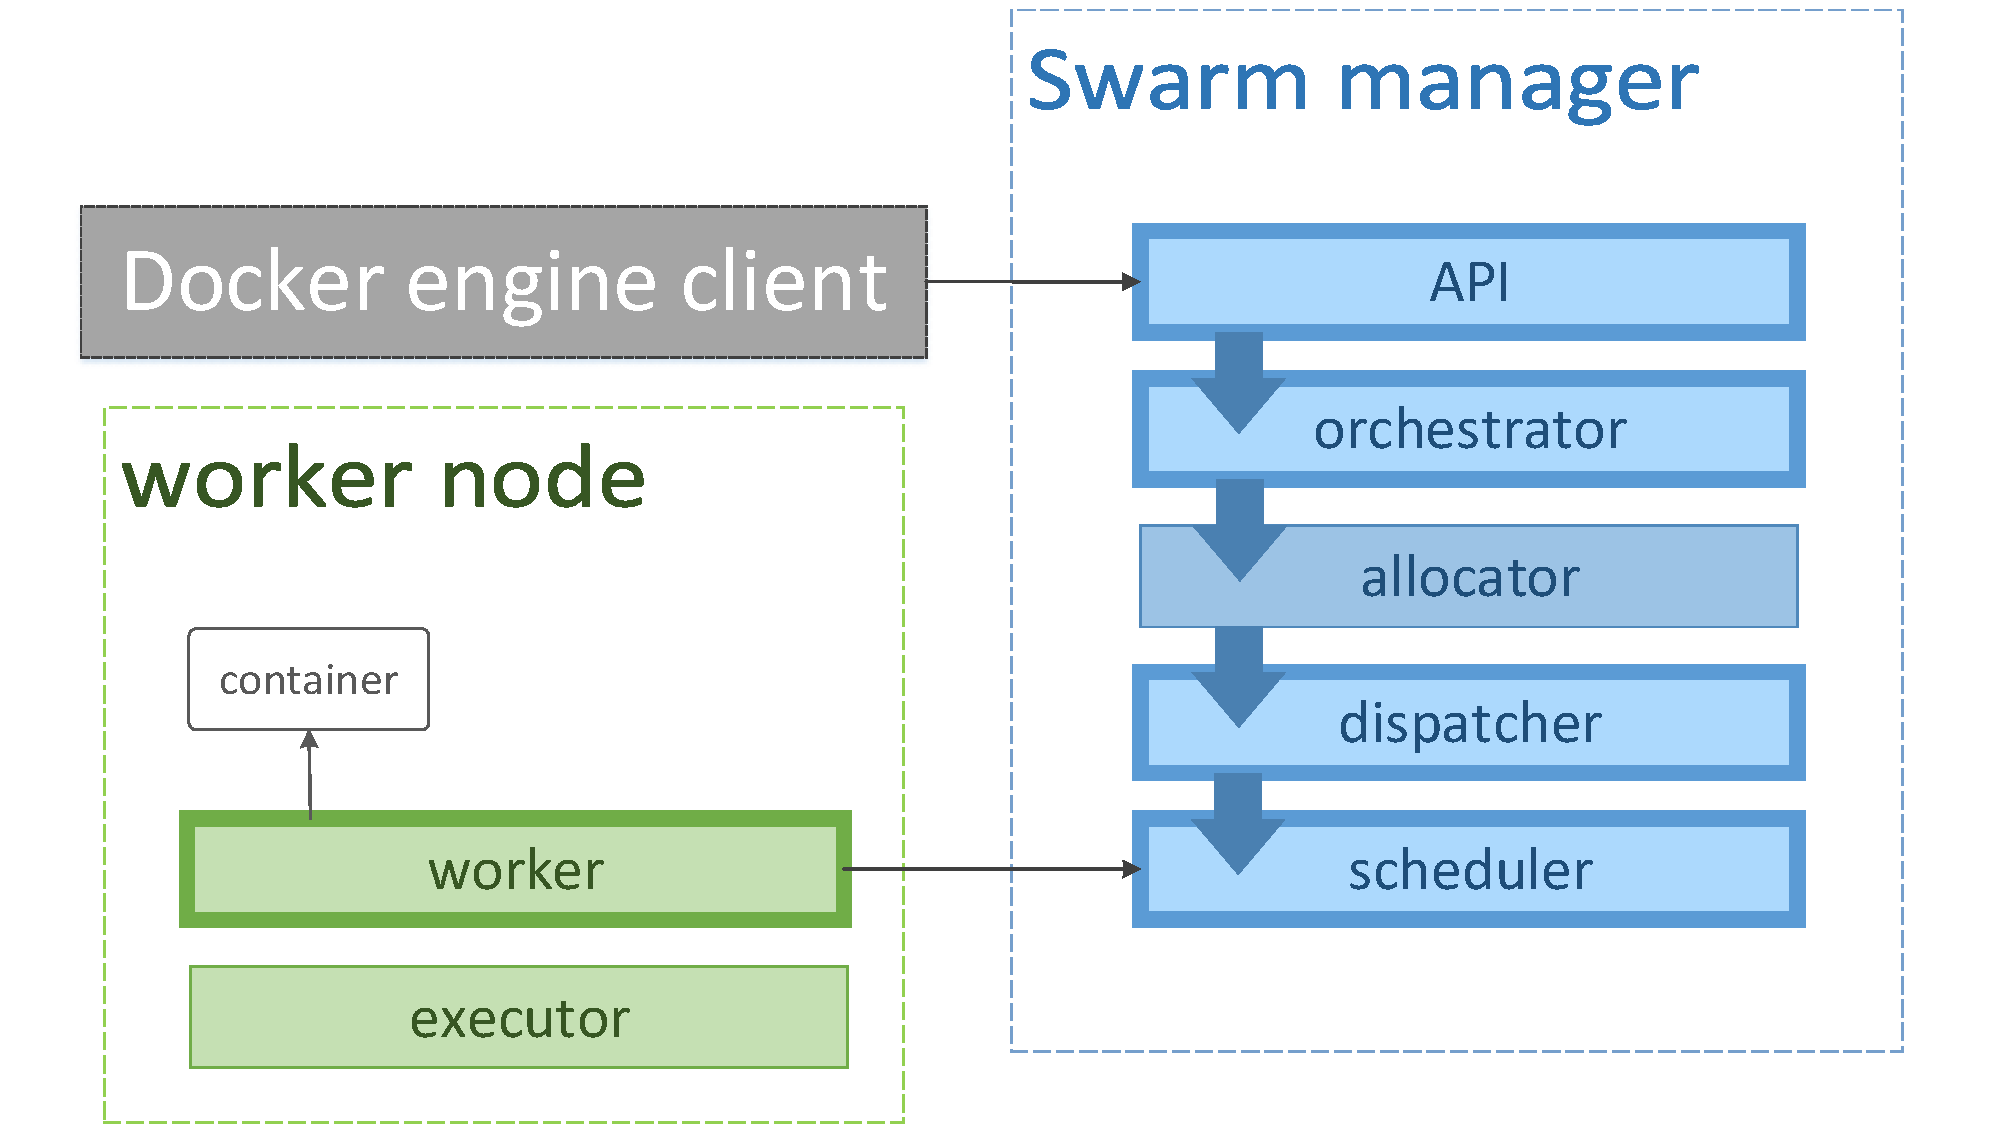
\includegraphics[width=0.9\textwidth]{./figure/modification}
\bicaption[fig:swarmkit-modify]{Docker中服务的运行流程}{\textbf{Docker中服务的运行流程}}{Fig}{How a service works in Docker \emph{swarm}}
\end{figure} 

整体而言,容器云中各个节点分为两种角色:管理者节点和工作者节点,其中管理者节点负责维护容器云中所有节点的信息并根据相应规则将任务的实例分发到相应的工作者节点之中,工作者节点在接受到分配的任务实例利用本节点的Docker Engine来启动容器运行相应的任务实例。对集群的一个节点而言,他必然是一个工作者节点,但是也可以有管理者节点的角色。

%\begin{figure}[!htp]
%    \centering
%    \resizebox{6cm}{!}{\input{figure/example/flow_chart.tex}}
%    \bicaption[fig:flow_chart]{绘制流程图效果}{流程图}{Fig}{Flow chart}
%\end{figure}

\section{资源使用状态监测模块}
图\ref{}显示了资源使用状态监测模块的详细类结构设计:

由图\ref{}可知,资源使用状态监测模块整体分为manager和worker两个部分,分别运行在容器云中的管理者节点和工作者节点上。

在工作者节点上,ResourceMonitor类通过调用getResourceUsageFromTasks方法基于容器中的资源监控接口周期性地获得该节点上所有任务实例的资源使用状态。为了增加可扩张性,方便用户后续加入其它资源属性,我们引入ResourceUsageAdapter接口,对资源使用状态进行采集并转换成符合设计部分中提到的数据格式。由于本系统基于Docker实现,我们用DockerResUsageAdapterImpl作为默认的ResourceUsageAdapter接口实现类,利用Docker中的状态接口获取各个任务实例和节点本身的资源使用状态,并将相应数据转换成符合本模块需要的格式。类DataStandardizer通过standardize方法对采集到的原始数据进行采样化处理,以3秒为周期对每个周期内的数据取均值后作为这段时间内的观测数据,以减小短时间内观测值的波动,降低整体的观测误差和传输的数据大小。随后,RawDataClient类利用syncRawData方法通过gPRC接口以30秒为周期,将工作节点上统计得到的数据发送给给管理者节点,发送的数据利用Protocol Buffers进行序列化,定义如代码中\ref{code:raw_format}所示:
\begin{lstlisting}[language=protobuf3,style=protobuf, caption={资源使用状态监测数据},label={code:raw_format}]
message ResourceUsage {
    int64 time = 1;
    float cu = 2;
    float ca = 3;
    int64 mu = 4;
    int64 ma = 5;
    int64 niu = 6;
    int64 nia = 7;
    int64 nou = 8;
    int64 noa = 9;
}

message TaskInfo {
    string taskID = 1;
    string serviceID = 2;
}

message RawData {
    ResourceUsage res = 1;
    oneof item {
        string nodeID = 2;
        TaskInfo task = 3;
    }
}
\end{lstlisting}
在管理者节点上,RawDataServer类利用syncRawData方法通过gPRC接口从工作者节点的RawDataClient类上接受相应的观测数据。在RawDataServer类获取监控数据之后,PredicatorMonitorProducer类和UtilMonitorProducer类分别负责将相应的资源使用状态监控数据通过gRPC接口发送给资源使用状态预测模块和资源供给优化模块。

\section{资源使用状态预测模块}
资源使用状态预测模块的类结构设计如图\ref{}所示:

我们使用gPRC的方式和资源使用状态监测模块建立RPC通信,PredicatorMonitorConsumer类负责从资源使用状态监测模块周期性地获取整个容器云中各个服务的资源使用状态数据。
资源使用状态预测模块主要负责根据不同的预测算法对历史数据进行预测,但是考虑到实际应用中云环境的复杂性,为了方便用户能够在将来根据自身需要选择其他的预测算法,因此使用抽象工厂的设计模式来实现不同预测处理类的创建,方便后续的扩展。PredicatorFamilyFactory接口中定义了createPreidcatorFamily方法,并通过此方法来生成支持的预测器族PredicatorFamily接口。PredicatorFamily接口通过getPredicator方法根据实际需要得到相应的Predicator接口,而Predicator接口则通过predicateNextPeriod方法利用PeriodNormalizer接口获取对下个周期的预测结果,最后利用PeriodNormalizer接口中的normalizePredication函数来获取一个周期内的最终数值调整。

在本系统中,默认支持基于经典时间序列预测算法和基于深度学习的预测算法,因此PredicatorFamilyFactory接口默认支持两个不同的工厂类型实现:ClassicFamilyFactory类和DeepLearningFamilyFactory类,分别对应基于经典时序数据模型的预测器工厂类型和基于深度学习模型的预测器工厂类型;ClassicPredicatorFamily类和DLPredicatorFamily类分别对应基于经典时序数据模型的预测器族类型和基于深度学习模型的预测器族类型;ARIMAPredicator类和LSTMPredicator类分别对应基于ARIMA模型的预测器类型和基于LSTM模型的预测器类型;DefaultPeriodNormalizer类为PeriodNormalizer接口的默认实现。

\section{资源供给方案生成模块}
资源供给方案生成模块的类结构设计如图\ref{}所示:

InstanceMapper类负责根据各个资源的使用量确定需要的任务实例个数,通过getInstancesBySpec方法获得满足资源需求的最少实例数。InstanceFlatter类负责对一个周期内所有的任务实例调整请求进行最终整理和梳理,通过getFinalInstance方法获得本周期内的最终确认的任务实例调整结果。最后,通过InstanceScheduler类的updateSchedule方法将基于预测的实例调整结果通过gRPC接口发送给资源管理模块。

\section{资源供给优化模块}
资源供给优化模块和资源供给方案生成模块在设计中比较相似,因此具体的实现也和资源供给方案生成模块实现很相近。资源供给优化模块中的类结构设计如图\ref{}所示:

UtilMonitorConsumer类负责利用心跳的机制通过gRPC接口从资源使用状态监测模块获取容器云中各个服务和节点的资源使用状态监测数据,ResUsageWatcher接口在resUsageWatch方法中通过检查过去三个周期内的资源使用量是否超过阈值来判断是否需要进行优化调整。当实际资源使用量超过扩展警戒阈值时,ResUsageWatcher接口通过emergentIncrease方法增加实例规模;当实际资源使用量收缩警戒阈值时,ResUsageWatcher接口通过emergentDecrease方法减小实例规模。在本文提出的系统,DefaultResUsageWatcher类是ResUsageWatcher接口的默认实现,使用模块设计中的调整算法。用户可以根据自身的需要,通过实现ResUsageWatcher接口来定制符合自身需要的动态调整方案。

\section{资源管理模块}
图\ref{}显示了资源管理模块中的类结构设计:

在资源管理模块中,ServiceAvailabilityCalculator接口通过getServiceReplica方法根据容器云中各节点的可用性指标和资源使用状态计算出服务需要的副本分布。本系统中ServiceAvailabilityCalculator接口的默认实现类为HomoServiceAvailabilityCalculator类,针对的是同构(即容器云中各节点的可用性指标都一样)的容器云,计算方法如设计中公式\ref{eq:replica}所示。GeneratorChanger类和UtilChanger类利用gRPC接口分别从资源供给方案生成模块和资源供给优化模块获取相应请求的实例规模,并将请求通过ScaleRequestQueue类的addScaleRequest方法将相应数据添加到相应的等待队列中。ServiceScaleHandler接口通过tick方法周期性的对等待队列进行遍历,将等待队列中的服务伸缩请求按照其中时间戳数据的先后顺序,利用本系统中修改的服务伸缩API依次发起服务伸缩请求。此外,资源管理模块通过ImageFSQuery类通过Docker \emph{registry} API获取服务运行所需Docker镜像中的层级文件信息,并保存在内存中。RootFSSync类通过gRPC接口将各个工作者节点上的层级文件缓存信息按照增量的方式周期性地同步到工作者节点中。

\section{负载优化模块}
负载优化模块中的类结构设计如图\ref{}所示:

ServiceHandler类负责接收所有的服务相关的请求,包括服务的创建请求、销毁请求和伸缩请求,并将请求转发给ABPScheduler类。ABPScheduler类对收到的所有服务变更请求放入等候队列中,通过tick方法周期性地对等候队列中的所有服务变更请求进行处理。根据服务请求的类型,ABPScheduler类利用createService方法来负责处理服务的创建请求,通过deleteService方法来负责处理服务的销毁请求,用scaleService方法来负责处理服务的伸缩请求。ABPScheduler类在scaleService方法中对当前服务的实例规模和请求的实例规模进行对比:如果请求的实例数超过当前实际的实例数,则ABPScheduler类通过scaleoutService方法对相应服务进行扩展;如果如果请求的实例数少于当前实际的实例数,ABPScheduler类就使用scaleinService方法对相应服务进行收缩;如果实例数要求不变,则抛弃此次调整请求。在ABPScheduler中,我们利用taskFitNode方法来判断一个集群节点是否满足任务实例运行的需要。DRFNode类表示一个可能的任务节点组,其中利用getDrfResource方法可以获得该任务节点组的优势资源,基于启发式的多优先级规则在compare方法中重新定义DRFNode对象的优先级比较方法。


\section{本章小结}
本章通过类图的方式详细介绍了本文所实现系统中各个模块的具体实现方式。由于本文提出的系统是一个分布式系统,因此我们引入了大量的异步操作和批处理操作,从而实现提高系统整体吞吐量和健壮性的目标。在具体实现过程中,我们将整体的可扩展性和可维护性作为重要目标,使得我们实现的系统可以在后续的工作中进行进一步地完善和发展,让用户根据自身的需求进行自主化定制成为可能。